% Matteo Kumar - Leonard Schatt
% Fortgeschrittenes Physikalisches Praktikum
% 4.Kapitel Versuchsauswertung

\section{Ensemble measurements}\label{sec:ensemble}

For the ensemble measurements the fourteen samples of rods of different lengths and widths were measured with unpolarized light and light of \ang{0} and \ang{90} polarization each. The measured spectra $I_m$ were corrected using a reference spectrum $I_r$ taken without a sample for each of the three polarization setups. The corrected spectra $I_c$ were thus calculated as
\begin{equation}
    I_c = \frac{I_m}{I_r}.
\end{equation}
Although a dark spectrum $I_d$ was taken as well, it was not used for this evaluation, since $I_m$, $I_r$ and $I_d$ converged to the same intensities for increasing wavelengths and therefore creating singularities when subtracting $I_d$ from both $I_m$ and $I_r$. This could be done since the values for $I_d$ were constant and small for the relevant parts of the wavelength scale. The corrected spectra can be seen in fig.~\ref{fig:unpol}, \ref{fig:pol0} and \ref{fig:pol90}. Using a gaussian function the wavelength for the maximum intensity $\lambda_{max}$ was calculated. All values can be found in tab.~\ref{tab:lamMaxUn},~\ref{tab:lamMax0} and \ref{tab:lamMax90}.

\begin{figure}
    \centering
    \begin{subfigure}{\textwidth}
        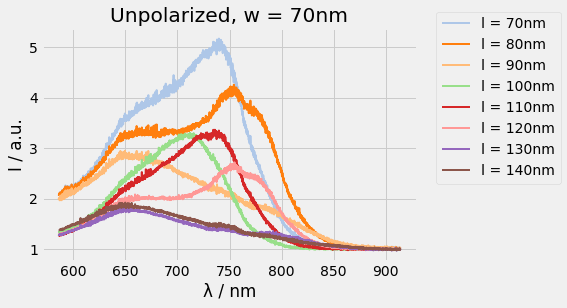
\includegraphics[width=\textwidth]{Bilder/Auswertung/SpektrumUnpol70.png}
        \caption{ }
        \label{fig:u70}
    \end{subfigure}
    \hfill
    \begin{subfigure}{\textwidth}
        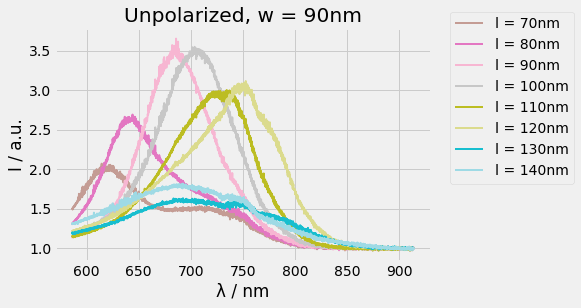
\includegraphics[width=\textwidth]{Bilder/Auswertung/SpektrumUnpol90.png}
        \caption{ }
        \label{fig:u90}
    \end{subfigure}
    \caption{The corrected spectra of the samples using unpolarized light are shown. While the rodlength varied throughput the samples, the rodwith of \SI{70}{\nano\meter} was fixed in (a) and one of \SI{90}{\nano\meter} in (b).}
    \label{fig:unpol}
\end{figure}

\begin{figure}
    \centering
    \begin{subfigure}{\textwidth}
        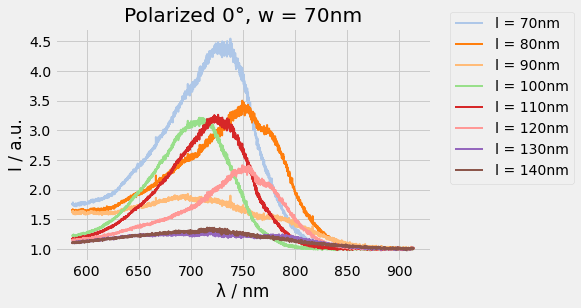
\includegraphics[width=\textwidth]{Bilder/Auswertung/SpektrumPol070.png}
        \caption{ }
        \label{fig:0-70}
    \end{subfigure}
    \hfill
    \begin{subfigure}{\textwidth}
        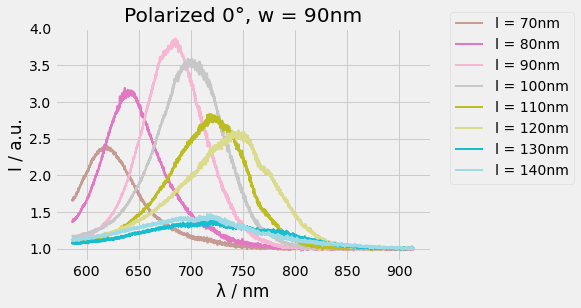
\includegraphics[width=\textwidth]{Bilder/Auswertung/SpektrumPol090.png}
        \caption{ }
        \label{fig:0-90}
    \end{subfigure}
    \caption{The corrected spectra of the samples using polarized light of \ang{0} are shown. While the rodlength varied throughput the samples, the rodwith of \SI{70}{\nano\meter} was fixed in (a) and one of \SI{90}{\nano\meter} in (b).}
    \label{fig:pol0}
\end{figure}

\begin{figure}
    \centering
    \begin{subfigure}{\textwidth}
        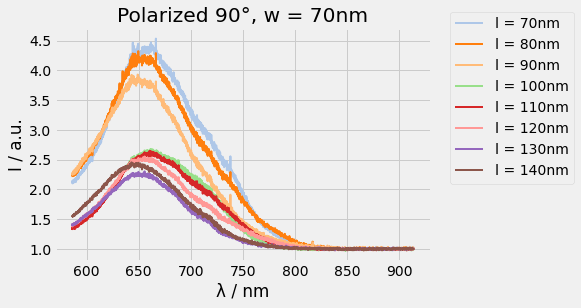
\includegraphics[width=\textwidth]{Bilder/Auswertung/SpektrumPol9070.png}
        \caption{ }
        \label{fig:90-70}
    \end{subfigure}
    \hfill
    \begin{subfigure}{\textwidth}
        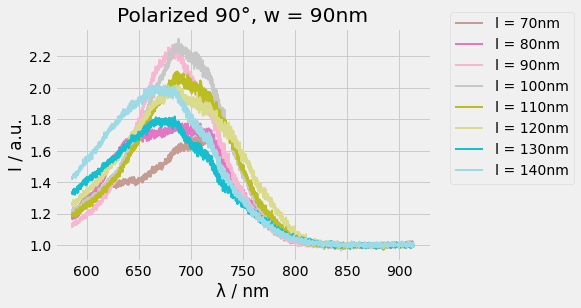
\includegraphics[width=\textwidth]{Bilder/Auswertung/SpektrumPol9090.png}
        \caption{ }
        \label{fig:90-90}
    \end{subfigure}
    \caption{The corrected spectra of the samples using polarized light of \ang{90} are shown. While the rodlength varied throughput the samples, the rodwith of \SI{70}{\nano\meter} was fixed in (a) and one of \SI{90}{\nano\meter} in (b).}
    \label{fig:pol90}
\end{figure}

\begin{table}
    \centering
    \begin{tabular}{c|cc}
        \toprule
        $l$ / \si{\nano\meter} &   $\lambda_{max,unpol,w=\SI{70}{\nano\meter}}$ / \si{\nano\meter}& $\lambda_{max,unpol,w=\SI{90}{\nano\meter}}$ / \si{\nano\meter}\\
        \midrule
        70  &  $708.2 \pm 0.4$&  $602.2 \pm 2.8$\\
        80  &  $741.5 \pm 1.0$&  $653.8 \pm 0.4$\\
        90  &  $669.6 \pm 0.3$&  $687.98 \pm 0.08$\\
        100 &  $696.44 \pm 0.18$&  $703.84 \pm 0.10$\\
        110 &  $712.5 \pm 0.3$&  $719.30 \pm 0.16$\\
        120 &  $757.6 \pm 1.4$&  $743.9 \pm 0.4$\\
        130 &  $668.5 \pm 0.4$&  $707.67 \pm 0.15$\\
        140 &  $664.8 \pm 0.3$&  $690.03 \pm 0.12$\\
        \bottomrule
    \end{tabular}
    \caption{Values of the wavelength of the maximum intensity of the spectra in fig.~\ref{fig:unpol}. All values were calculated from a fit using a gaussian function. The error represents the fitting error.}
    \label{tab:lamMaxUn}
\end{table}

\begin{table}
    \centering
    \begin{tabular}{c|cc}
        \toprule
        $l$ / \si{\nano\meter} &   $\lambda_{max,\ang{0},w=\SI{70}{\nano\meter}}$ / \si{\nano\meter}& $\lambda_{max,\ang{0},w=\SI{90}{\nano\meter}}$ / \si{\nano\meter}\\
        \midrule
        70 &  $715.1 \pm 0.3$&  $619.92\pm 0.15$\\
        80 &  $752.4 \pm 0.9$&  $642.88\pm 0.11$\\
        90  &  $688.1\pm 0.3$&  $683.02\pm 0.05$\\
        100 &  $700.21\pm 0.16$&  $699.07\pm 0.09$\\
        110 &  $716.48\pm 0.19$&  $716.39\pm 0.12$\\
        120 &  $751.4\pm 0.6$&  $736.7\pm 0.2$\\
        130 &  $709.5\pm 0.4$&  $715.3\pm 0.2$\\
        140 &  $705.8\pm 0.2$&  $699.33\pm 0.17$\\
        \bottomrule
    \end{tabular}
    \caption{Values of the wavelength of the maximum intensity of the spectra in fig.~ \ref{fig:pol0}. All values were calculated from a fit using a gaussian function. The error represents the fitting error.}
    \label{tab:lamMax0}
\end{table}

\begin{table}
    \centering
    \begin{tabular}{c|cc}
        \toprule
        $l$ / \si{\nano\meter} & $\lambda_{max,\ang{90},w=\SI{70}{\nano\meter}}$ / \si{\nano\meter}& $\lambda_{max,\ang{90},w=\SI{90}{\nano\meter}}$ / \si{\nano\meter}\\
        \midrule
        70  &  $664.06\pm 0.11$&  $687.18\pm 0.4$\\
        80  &  $659.13\pm 0.12$&  $678.41\pm 0.17$\\
        90  &  $651.89\pm 0.08$&  $684.50\pm 07$\\
        100 &  $668.10\pm 0.08$&  $690.46\pm 0.13$\\
        110 &  $668.06\pm 0.11$&  $691.38\pm 0.11$\\
        120 &  $660.99\pm 0.13$&  $688.20\pm 0.10$\\
        130 &  $653.20\pm 0.07$&   $668.06\pm 0.11$\\
        140 &  $649.43\pm 0.06$&  $664.28\pm 0.09$\\
        \bottomrule
    \end{tabular}
    \caption{Values of the wavelength of the maximum intensity of the spectra in fig.~\ref{fig:pol90}. All values were calculated from a fit using a gaussian function. The error represents the fitting error.}
    \label{tab:lamMax90}
\end{table}


    
As well in fig.~\ref{fig:pol90} as in tab.~\ref{tab:lamMax90} can be seen that in the case of a polarization of \ang{90} the wavelength at the maximum of the intensity spectra does not shift with a varying rodlength. This corresponds to the literature which lets us expect no shifting of the maxima only for the longitudinal modes~\cite{LehrstuhlExperimentalphysikIII.2023}. On the other hand, for the transversal modes (i.e.~a polarization of \ang{0}), a shift of the maximum can be observed in fig.~\ref{fig:pol0} and in tab.~\ref{tab:lamMax0}, both. The unpolarized spectra should show characteristica of transversal and longitudinal modes, as both are excited. This is the case here, as can be seen especially for $w$ = \SI{90}{\nano\meter} (and e.g.~$l$ = \SI{80}{\nano\meter}). Hereby can be seen, that the peaks for the longitudinal modes are smaller as the ones of the transversal modes.
% maxima 0 unpol correspond